Eine flache Platte ist um eine feste Achse durch D drehbar, die senkrecht zur Platte steht. Drei Kräfte wirken auf sie, gezeichnet auf einem Gitter aus Kästchen von \SI{10}{\cm}:
\begin{itemize}
 \item $F_1 = \FaO$ nach oben, Angriffspunkt 3 Kästchen rechts von D,
 \item $F_2 = \FbO$ nach rechts, Angriffspunkt 4 Kästchen rechts von und 1 Kästchen über D,
 \item $F_3 = \FcO$ nach unten, Angriffspunkt 5 Kästchen links von D.
\end{itemize}
\begin{center}
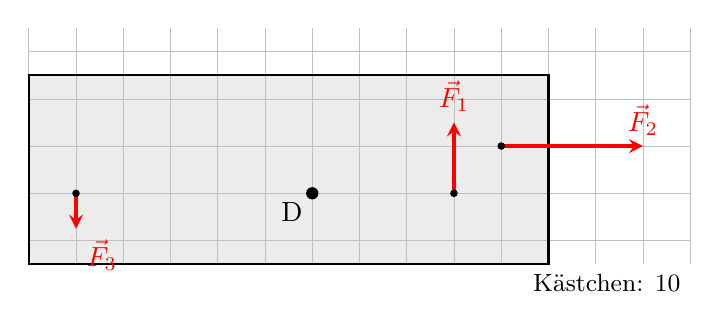
\begin{tikzpicture}[scale=0.6, >=stealth]
 \fill[gray!15] (-6,-1.5) -- (5,-1.5) -- (5,2.5) -- (-6,2.5) -- cycle;
 \draw[gray!50, very thin] (-6,-1.5) grid (8,3.5);
 \draw[thick] (-6,-1.5) rectangle (5,2.5);
 \fill (0,0) circle (0.13) node[below left] {D};
 \draw[->, very thick, red] (3,0) -- (3,1.5) node[above] {$\vec F_1$};
 \draw[->, very thick, red] (4,1) -- (7,1) node[above] {$\vec F_2$};
 \draw[->, very thick, red] (-5,0) -- (-5,-0.75) node[below right] {$\vec F_3$};
 \foreach \p in {(3,0),(4,1),(-5,0)} \fill \p circle (0.08);
 \node[below left] at (8,-1.5) {\small Kästchen: \SI{10}{\cm}};
\end{tikzpicture}
\end{center}

\begin{abcliste}
\abc
Ordne die Drehmomente der drei Kräfte bezüglich D nach ihrem Betrag, das kleinste zuerst. Gib auch den Drehsinn jeder Kraft an.

\abc
Lea ordnet einfach nach der Grösse der Kräfte. Tim ordnet nach dem Produkt aus der Kraft und dem Abstand von D zum Angriffspunkt. Zu welchen Reihenfolgen kommen die beiden, und was ist jeweils falsch?
\end{abcliste}
